\chapter{Empirical Study}
\label{chapter7}

In this chapter we will suplement our theoretical investigation of the w-structures with an empirical study. The goal of this study if twofold. Firstly it is to verify the theoretical claims we have made on the correctness and running time of the w-diameter algorithms we developed. This will be done by implementing and testing them on a range of datasets. The second goal and most important goal of the empirical study is to analyse the w-structures that are present in contour trees of real life data sets using the w-diameter algorithms we have implemented.

\section{Algorithm Implementations}

For the purpose of conducting the empirical study we implemented all three w-diameter algorithms we developed in Chapter []. Those are the brute force algorithm (NxBFS), the 2xBFS and DP algorithms.  We implemented the brute force algorithm by running the modified version of 2xBFS from every vertex in the tree and outputting the largest w-path we found. The implementation of the 2xBFS algorithm was based entirely on the pseudocode we provided in Chapter []. Initially we made a recursive implementation of the DP algorithm based on the pseudocode we provided in Chapter []. This approach was not efficient enough because the recursion added a substantial amount of overhead and slowed down computation on large data sets. We resorted to converting our recursive solution to an iterative one.

When converting a dynamic programming algorithm from a recursive to an iterative solution one first identifies all base case subproblems and solves them. Afterwards one works their way up to subproblems that depend only on the base case solutions and solve those. This process is repeated until all subproblems are solved. In our particular example the base cases are the leafs of the tree. The subproblems that depend on those are the vertices whose distance from a leaf is one. Once those are solved we move on to vertices whose distance from a leaf is two and so on.

To begin with we first have to root the tree using a standard Breath First Search. The root of the tree can be any vertex. Using the BFS we not only assing parrents to all vertices, but we also rank them based on their distance from the root. By processing vertices from furthest to the root inself we ensure that the subproblems of any vertex are solved for because its children have a bigger distance. In order to solve a subproblem at a vertex we can use the code we have provided in the backtracking part of the DFS in the pseudocode in Chapter [].

Finally we also implemented the serial contour tree algorithm as it is described in []. The reason for doing so is that we needed to use it to compute the contour tree of test data and then execute the w-diameter algorithms of those contour trees. This required us to make some modifications in the output of the contour tree algorithm to better suit the expected input of the w-diameter algorithms. All four algorithms we devloped were written in C++ and their source code can be found in their github repository [].

\section{Data sets Overview}

Before describing our testing methodology we will first elaborate on the types of data sets we will be using throughout our tests. The first type of data sets we will use are randomly generated height trees. In testing the correctness and running time of the w-diameter algorithms we would ideally like to run them on as many different data sets as possible in order to confirm our theoretical claims for all of them. Generating height trees randomly will allows us to produce new data sets for testing on demand. We will now describe the algorithm we implemented for generating random trees.

Starting with a disconnected graph $G$ with $n$ vertices we generate pairs of vertices $u, v$ in with random labels generated uniformly in the range $\{1, 2, ..., n\}$. If adding the edge $uv$ to the graph does not create a cycle we keep the edge. If it does create a cycle we discard it. We continue generating edges untill the $G$ is fully connected. Upon reaching this point $G$ will be a connected graph with no cycles. This is exactly the definition of a tree. In order to produce valid height trees we assign a random height to each of the vertices of the tree. In order to detect whether adding an edge produces a cycle we use the union-find data structure to keep track of which connected components vertices belong to. We add an edge between two vertices only when they belong to a different connected component and then merge the two components together.

The second type of data sets we will use is real life data taken from the GTOPO30 data set. GTOPO30 [] is a digital elevation model of the world. The dataset is a two dimensional data grid containing the elevation of points on Earth with a resolution of approximately one kilometer. The primary use of this data set will be for the contrusting a contour tree of it and analysing the present w-structures. GTOPO30 however is far to large for us to handle without specialised hardware. This is why we have taken several smaller subsets of GTOPO30 provided to us by Dr. Hamish Carr.

Our data sets are chosen based on their their topographic complexity. All of them are both mountainous and lowland regious in Canada. The data sets we will use are named vanc (18x21), vancouverSWSW (25x49), vancouverSWNE (25x50), vancouverSWNW (25x50), vancouverSWSE (25x51), vancouverNE (49x99), vancouverNW (49x100), vancouverSE (50x99), vancouverSW (50x100), icefields (240x240), pukaskwa (551x1600) and gtopo30w020n40 (6000x4800). The vanc and all other vancouver data sets are taken from the North Shore Mountains that overlook Vancouver in British Columbia, Canada. The data set pukaskwa is taken from the Pukaskwa National Park located south of the town of Marathon, Ontario, Canada. The data set icefields straddles the contitnental divide. It is taken from Icefields Parkway in the heart of the Canadian Rocky Mountain. Finally gtopo30w020n40 is the data set that contains all other data sets.

\section{W-detector Algorithms}

In this section we will use our implementations of the NxBFS, 2xBFS and DP algorithms to empirically test whether our claims on their correctness and running time are correct. The first test we will present is on the correctness of all three algorithm. The major issue we encountered in this test is that all three algorithm solve a problem that to our knowledge has not been been considered extensively. The only way to establish ground truth on their output is to manually inspect the w-diameter of a height tree. This is neither reliable nor scalable to height trees with more than a few dosen vertices.

To overcome this issue we opted for using the output of the NxBFS algorithm as ground truth. The reason is that it is the most straighforward to implement and that its correctness is a trivial consequence of its formulation. We belive that this makes it the most reliable of the three. A further complication arises with the fact the NxBFS algorithm's running time is quadratic and not linear like 2xBFS and possibly DP. This leaves us unable to use this methodology for large enough trees where the NxBFS algorithm's computation simply scales to unreasonable time. This is why we have limited ourselves to only testing correctness for trees of up to 10,000 vertices. For this test we have used the following testing methodology:

\begin{itemize}
    \item Generate a random tree.
    \item Run all three algorithms on the tree.
    \item Check whether the output of DP and NxBFS are the same and if the output of 2xBFS is within two of their output.
\end{itemize}

We then used this methodology to run tests on one thousand trees of sizes $50$, $100$, $250$, $500$, $750$, $1000$, $2500$, $5000$, $7500$, $10000$ resulting in $10000$ individual tests alltogether. The output of all tests was in line with what we predicted in Chapter 3. The algorithms DP and NxBSF had identical output and the output of the 2xBSF algorithm was no less than two of their output. These results strengthen our belief in the correctness of all three algorithms.

The second test we will perform is on the running times of the algorithms. The algorithms will be separated in two groups. The first group will contain NxBFS and the second group will contain 2xBFS and DP. We have separated them because we expect the running time of NxBFS to be quadratic, 2xBFS to be linear, DP to be close to linear and we want to results within each group to be comparable. The results from testing the NxBSF algorithm were completely as expected. You can see the running time on Figure \ref{fig:nbfs}. As expected it fits a quadratic curve.

\begin{figure}[h]%
    \centering
    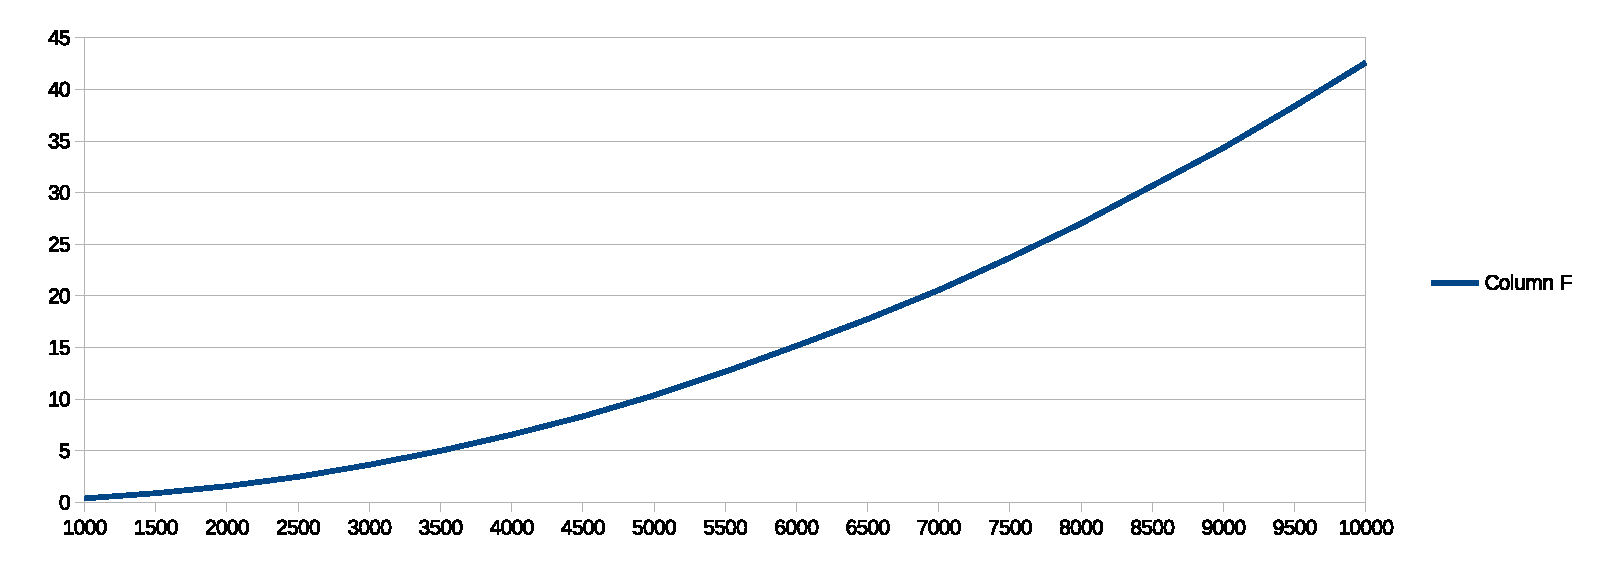
\includegraphics[center, scale=0.6 ]{./images/empirical/chart-nbfs.eps}
    \caption{Running time of NxBFS on randomly generated trees. }%
    \label{fig:nbfs}%
\end{figure}


The test of the running time of the 2xBFS and DP algorithms provided more insight. The test consisted of generating five trees per tree size in the range of $\{5000, 10000, 15000, ..., 200000\}$. We ran both algorithms on all five trees for all tree sizes totalling 195 tests altogether. We plotted the average running time across all five trees per tree size on Figure \ref{fig:2xbfs-dp}. This chart shows that the peformance of both 2xBFS and DP scales linearly with randomly generated height trees in the $[5000, 200000]$ vertex range.

This comes as no suprise as regards to the 2xBSF algorithm. We showed that its running time is linear. What is interesting to see is that the DP algorithm's performance scales linearly as well. We must note however that these tests use randomly generated trees and are a very limited sample so this trend may not hold for all possible inputs and especially for larger trees. Despite these reservations this test gives credibility to the claim we made in the Chapter [] that the DP algorithm has potential for good practical performance despite its quadratic worst case time complexity.

\begin{figure}[h]%
    \centering
    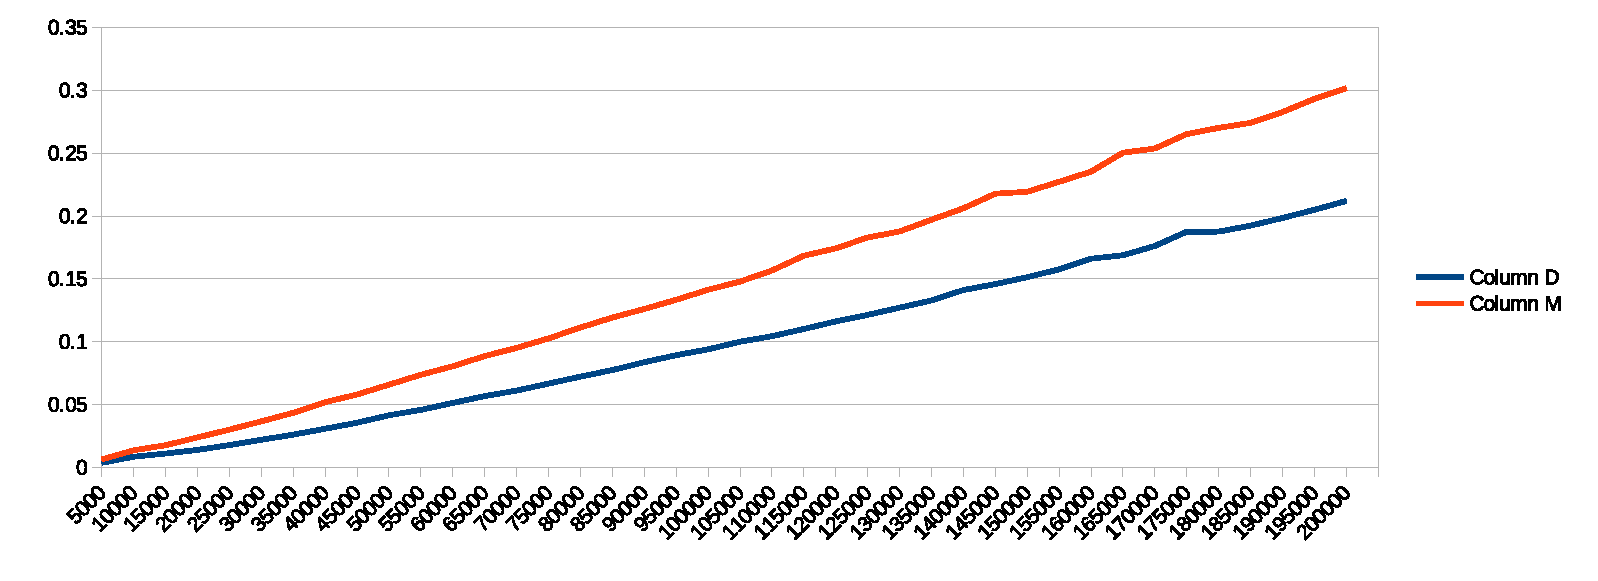
\includegraphics[center, scale=0.6 ]{./images/running-time-new.eps}
    \caption{Running time of 2xBFS (blue) and DP (red) on randomly generated trees. }%
    \label{fig:2xbfs-dp}%
\end{figure}


% Our next test was again on the running time of the algorithm but on the real data sets. The tests were run on the augmented contour tree of the datasets.

The next test we made was on the running time of the algorithms on the GTOPO30 data sets. We ran the tests for both the augmented and unaugmented contour trees and recorded how many time times faster 2xBFS is than DP in the Factor column of the tables.

% 25.60 Товарителница 800044202201

\begin{center}
\begin{tabular}{l*{6}{c}r}

Dataset            & Vertices        & 2xBFS              & DP                   & Factor \\
\hline
vanc	           & 378	         &0.000413	          & 0.000497	         &1.20    \\
vancouverSWSW	   & 1225	         &0.000918	          & 0.002317	         &2.52    \\
vancouverSWNE	   & 1250	         &0.000937	          & 0.001858	         &1.98    \\
vancouverSWNW	   & 1250	         &0.000798	          & 0.002454	         &3.08    \\
vancouverSWSE	   & 1275	         &0.001009	          & 0.00204	             &2.02    \\
vancouverNE	       & 4851	         &0.003637	          & 0.005493	         &1.51    \\
vancouverNW	       & 4900	         &0.002893	          & 0.005612	         &1.94    \\
vancouverSE	       & 4950	         &0.002958	          & 0.005863	         &1.98    \\
vancouverSW	       & 5000	         &0.002795	          & 0.005658	         &2.02    \\
icefield	       & 57600	         &0.036430	          & 0.066978	         &1.84    \\
pukaskwa	       & 881600	         &0.520608	          & 0.962897	         &1.85    \\
gtopo30w020n40	   & 28800000	     &19.103233	          & 34.427916	         &1.80    \\

\end{tabular}
\end{center}

The results from this test are completely in line with what we obtained in Figure \ref{fig:2xbfs-dp}. The linear relationship between the running times of two still holds. DP is within the range of 1.2 - 3 times slower than the 2xBSF algorithm. In our next test we tested the same data sets, but we computed their unaugmented contour tree.

\begin{center}
\begin{tabular}{l*{6}{c}r}
Dataset                & Vertices                    & 2xBFS                             & DP                    & Factor \\
\hline
vanc	               & 29    	                     & 0.000136	                         & 0.000057	              & 0.42  \\
vancouverSWSW	       & 58   	                     & 0.000372	                         & 0.000127	              & 0.34  \\
vancouverSWNE	       & 148  	                     & 0.000355	                         & 0.000237	              & 0.67  \\
vancouverSWNW	       & 88   	                     & 0.000412	                         & 0.000163	              & 0.40  \\
vancouverSWSE	       & 109  	                     & 0.000351	                         & 0.000193	              & 0.55  \\
vancouverNE	           & 946    	                 & 0.001888	                         & 0.001730	              & 0.92  \\
vancouverNW	           & 911    	                 & 0.001505	                         & 0.001292	              & 0.86  \\
vancouverSE	           & 782    	                 & 0.001466	                         & 0.001107	              & 0.76  \\
vancouverSW	           & 380    	                 & 0.001756	                         & 0.000802	              & 0.46  \\
icefield	           & 7655  	                     & 0.013704	                         & 0.010280	              & 0.75  \\
pukaskwa	           & 65826 	                     & 0.183262	                         & 0.100899	              & 0.55  \\
gtopo30w020n40	       & 2436622 	                 & 6.609592	                         & 3.742080	              & 0.57  \\

\end{tabular}
\end{center}

The results here are quite suprising and they requried us to double check the test multiple times. On the outlook it seems that the two algorithms had exchanged their positions. The DP algorithm is 1.2 - 3 times faster than the 2xBFS algorith on all data sets. We are curious to know why this is the case. The difference between the augmented and the unaugmented datasets is that in the unaugmented datasets all vertices of degree two are removed. It would appear to be the case that such vertices are processed faster by the 2xBFS algorithm and the DP algorithm has some overhead associted with them.


% *I'll leave this paragarph and expand it if I have extra space*. Finally we would like to present a special case where the DP algorithm perform poorly. This case is for trees with vertices of high degree. Take for example a type of tree called a start Figure []. The doubly nested loop of the algorithm causes quadratic performance. To test this we generated a number of star like trees and compared the performance of NxBFS and DP.

% As we can see the results are again consistent with what we had with the random data sets.
%
% Except for gtopo30w020n40 where for some reason it's the other way around!!!
%
% Maybe it's the number of leaves? But it doesn't seem that way.


\section {Dataset w-diameter analysis}

In this section we will examine w-structures present in real data sets. Our goal is to demonstrate that they not only pose a theoretical difficulty, but also hinder practical performace. In this study we will execute our w-diameters algorithm on the mountain range data taken from GTOPO30. We will compare the w-diameters we obtained from the contour trees of the data sets with the diameters of the unaugmented and the augmented contour trees. We will demonstrate that w-diameter of a contour tree is a better theoretical upper bound on the time complexity of the parallel contour tree algorithm than either of the two diameters.

Secondly we will compare the w-diameter of a contour tree with the number of iterations that are need to collapse the join and split trees. We hope to find a correlation between the two that would support our theoretical claim that the it is the largest w-structure in a contour tree that prevents logarithmic collapse in the merge phase. We have taken the number of iterations needed to merge the join and split tree by running an implementation of the data-parallel contour tree algorithm based on [] provided to us by Dr. Hamish Carr [].

\begin{center}
\begin{tabular}{l*{6}{c}r}
Dataset             & 2BFS  & DP    & NBFS    & Aug Diameter  & Diameter  & Iterations\\
\hline
vanc                & 2     & 2     & 2       & 311           & 11        & 2  \\
vancouverSWSW       & 2     & 2     & 2       & 845           & 17        & 3  \\
vancouverSWNE       & 5     & 5     & 5       & 423           & 34        & 4  \\
vancouverSWNW       & 3     & 3     & 3       & 712           & 23        & 3  \\
vancouverSWSE       & 3     & 3     & 3       & 759           & 30        & 3  \\
vancouverNE         & 4     & 5     & 5       & 1338          & 128       & 5  \\
vancouverNW         & 5     & 5     & 5       & 1456          & 98        & 5  \\
vancouverSE         & 6     & 6     & 6       & 1306          & 118       & 5  \\
vancouverSW         & 4     & 4     & 4       & 1977          & 48        & 4  \\
icefield            & 7     & 7     & 7       & 12280         & 886       & 6  \\
pukaskwa            & 180   & 180   & N/A     & 374866        & 1046      & 94 \\
gtopo30w020n40      & 8     & 8     & N/A     & 15766966      & 305290    & 8  \\

\end{tabular}
\end{center}

%@TODO Remove the equiv
The first infrence we can make is about the pukaskwa data a set. Both the w-diameter and number of iterations are drastically bigger than all of the other data sets. If logarithmic collapse was taking place in the merge phase of the construction of the contour tree of pukaskwa then we would expect that to take $log_2(881600) \equiv 19$ iterations. Instead it takes $94$ iterations. This is consistent with the w-diameter of the data set. Indeed the w-diameter at $180$ kinks is almost twice as big as the number of iterrations $94$. If we consider that the algorithm can process two branches on oposite sides of the w-diameter at a time it makes sense that it should take twice as less iterations for the collapse if it were w-diameter that is causing it.

Secondly, we can confirm that the w-diameter in almost all of the data sets (except for vancouverSWSW) is bigger than or equal to the number of iterations. This leads us to believe that the two may be correlated. In the case of pukaskwa we have already given an interpretation of this corelation. By that reasoning we would expect that in other data sets the w-diameter to be twice as much as the number of iterations. This is not the case and this may very well be due to how different w-structures interact in the merge phase. This is something we have not investigated as we only record the largest w-structure.

% Another interesting thing to note is that pukaskwa is a subset of the gtopo30w020n40 dataset and yet it's w-diameter is far smaller. This proves that the contour trees of subsets of data need not have a smaller w-diamete. Strangely enough as a consequence of this subsets of data may not be faster to compute. This has

Fillay we turn our attention to the diameter of the augmented and unaugmented contour trees. The parallel contour tree algorithm currently uses those as an uppen bound on the time complexity of the merge phase []. We have already shown theoretically that the w-diameter of a height tree is necessarily smaller than its diameter. This empirical study demonstrates the practical relevance of this findind. In the most extreme example, that of gtopo30w020n40, the w-diameter of the augmented contour tree is 1,970,870 times smaller than its diameter. For all practical intents and purposes this is a huge difference. If the w-diameter of that data sets were equal to the actual diameter, than we would expect the merge phase to take a far larger number of iterations and severly limit the available parallelism in it.

% \section{Generating W-Structures Manually}
%
% % We can generate them via ridges and valleys.
% The next step we shall take in improving our understanding of the w-structures empirically will be to devise a way of creating data sets whose contour trees have an arbitrarily large w-diameter. In order to do so we took an approach of exhaustive enumeration. We limited ourselves to two dimensional data sets of dimension 3x3. Enumerating larger two dimensional data sets or almost any three dimensional data sets would not be feasible due to the number of permutations required. We created a program that generated all permutations of the numbers $1, 2, 3, 4, 5, 6, 7, 8, 9$ and arraged them in a 3x3 grid. After genrating all permutation we computed their contour tree and inspected the ones with maximum w-diameter. In our findings we discovered that there is a particular pattern in two dimensional data grids that can exploited to generate arbitrarily large w-structures. As an example consider our familiar simplicial mesh and contour tree on Figure [].
%
% % Here is an example data set and it's contour tree.
%
% % The data set consists of ridge and valleys.
%
% % This led us to find a pattern. Consider the data set.
%
% % \[
% %  \begin{matrix}
% %   1 & 0 & 1 \\
% %   0 & 1 & 0 \\
% %   1 & 0 & 1
% %  \end{matrix}
% % \]
%
%
% \begin{figure}[h]%
%     \centering
%     \subfloat[Simplicial Mesh]{{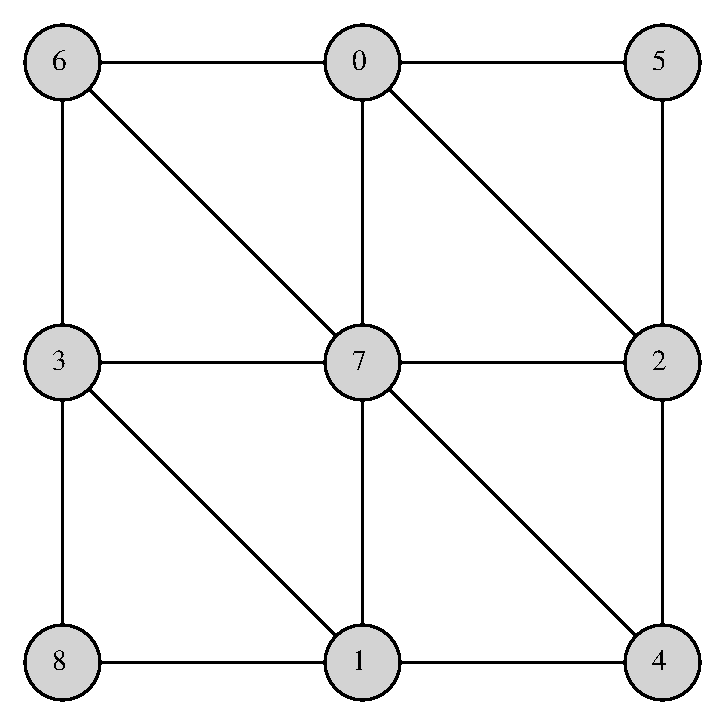
\includegraphics[scale=0.4]{./images/chapter4/w3x3-grid.eps}}}%
%     \qquad
%     \subfloat[Contour Tree]{{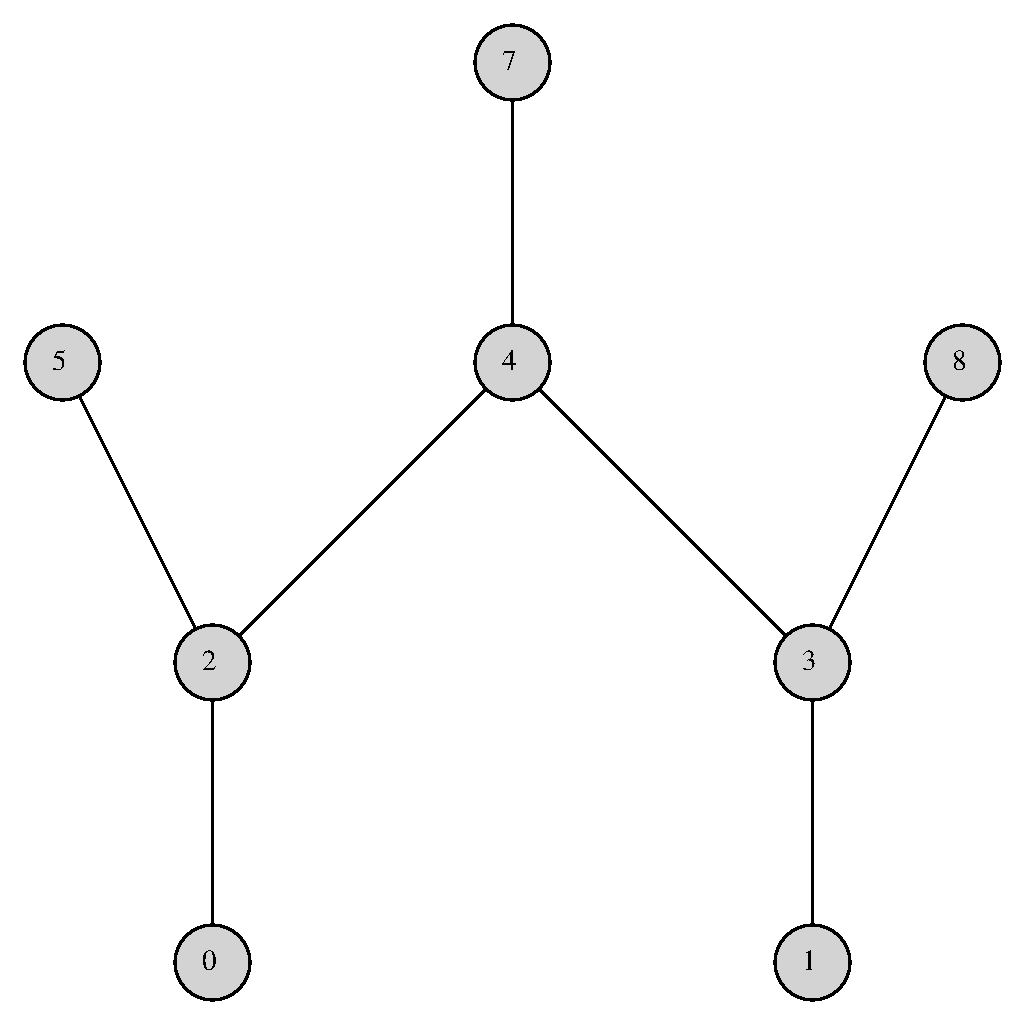
\includegraphics[scale=0.3]{./images/w3x3.eps}}}%
%     \caption{Simplicial Mesh of a Contour Tree}%
%     \label{fig:example}%
% \end{figure}
%
% The pattern in this simplicial mesh that is responsible for the w-diameter of three is a series of diagonal ridges and valleys. We can describe it like so:
%
%
% \[
%  \begin{matrix}
%   1 & 0 & 1 \\
%   0 & 1 & 0 \\
%   1 & 0 & 1
%  \end{matrix}
% \],
%
% where the ones represent vertices with heights bigger than the vertices labeled as zero and the relative height between of vertices with label one (or zero) does not matter. In order to expand the w-diameter by one we must extend the data set with an additional column.
%
% \[
%  \begin{matrix}
%   1 & 0 & 1 & 0 \\
%   0 & 1 & 0 & 1 \\
%   1 & 0 & 1 & 0
%  \end{matrix}
% \]
%
% The resulting contour tree of this data set would be.
%
% \begin{figure}[h]%
%     \centering
%     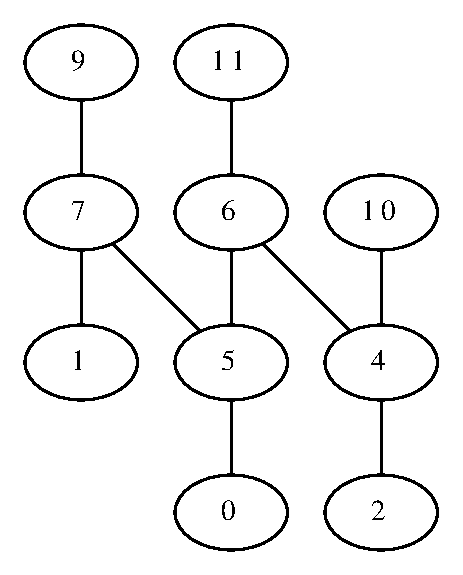
\includegraphics[center, scale=0.6 ]{./images/tree.eps}
%     \caption{Contour Tree of Dataset [] }%
%     \label{fig:case1.1}%
% \end{figure}
%
% After extending the data set for example to a 3x10 data set we obtain the following:
%
% \[
%  \begin{matrix}
%   1 & 0 & 1 & 0 & 1 & 0 & 1 & 0 & 1 & 0 \\
%   0 & 1 & 0 & 1 & 0 & 1 & 0 & 1 & 0 & 1 \\
%   1 & 0 & 1 & 0 & 1 & 0 & 1 & 0 & 1 & 0
%  \end{matrix}
% \]
%
% This 3x10 data set results in a contour tree with a w-diameter of ten on Figure [].
%
% \begin{figure}[h]%
%     \centering
%     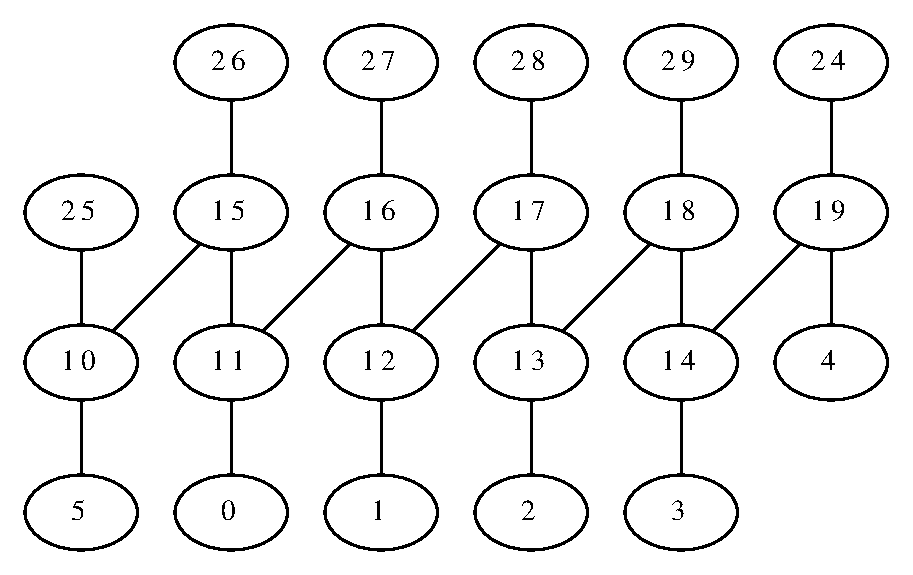
\includegraphics[center, scale=0.6 ]{./images/tree10.eps}
%     \caption{Contour Tree of Dataset [] }%
%     \label{fig:case1.1}%
% \end{figure}


% Can be obtain the w-diameter from raw data?

% Can we generate them in other ways?




% In this chapter we will study the w-structures empirically by implementing the algorithms that we can developed in Chapter \ref{chapter2} and using them to analyse real world data sets. The reason for studying them in practise is to learn more about them and explore how exactly they slow down computation. To accomplish this we will set two primary objectives. Firstly to correlate the iterations needed to collapse the contour tree in the merge phase of the algorithm with its w-diameter. This aims to give strength to the hypothesis that the w-structures do slow down computation in practise. Secondly to demonstrate that w-structures are found in real world data and do appear more abundantly as the size of datasets increases.
%
% In addition to out primary objectives there are some additional topics, related to the empirical study, that will be explored
%
% \begin{itemize}
%     \item Description the implementation of all used algorithms.
%     \item Demonstration of the running time of the implementations of the algorithms.
%     \item Correlating iterations for collapse with w-diameter of randomly generated tree.
%     \item Determining the smallest 2-dimensional grid dataset that exhibits a w-structure.
%     \item Discussion on the kinds of structures in raw data that produce w-structures in the contour trees.
%     \item Discussion on whether it is possible to determine the w-diameter of a datasets without computing it's contour tree beforehand.
%     %\item Exploring the statistical distribution of w-structures in randomly generated trees.
% \end{itemize}

%The first step to overcoming a problem is to learn about it. We .
%As a result of this study we will be able to shed light on the practical obstacles that the w-structures pose.

% For the purpose of the empirical study we implemented all three w-diameter algorithms we developed in the previous chapter. Those are the brute force algorithm, the 2xBFS and DP algorithms. In order to produce the contour trees of real life data sets we also implemented the serial version of the contour tree algorithm that is based directly on \cite{carr-masters}. To test our implementations for correctness we required the generations of more data sets than we had. This is why we have also written three small utility programs. One generates randomly populated data grids of size $n \times m$, the second generates random trees on $n$ vertices and lastly one that generates all $n \times m$ permutations of data grids populated with the numbers from $1$ to $n \times m$.  All algorithms were implemented in C++ and all algorithms are serial.
%
% The first algorithm that we implemented was the algorithm for computing the contour tree. To keep the implementation of this algorithm straightforward we have opted for working with two dimensional data sets only. To ensure the correctness of the implementation we have ran the code against code provided by Dr. Hamish Carr that implements the same algorithm. We have found that the two implementations produce the same output for all data sets we have tested - both from real data and random data.
%
% For the brute force algorithm and the 2xBFS algorithms we based our implementation entirely on the pseudocode provided in the previous chapter. The source code for those can be found in the appendix. For the DP algorithm we had to implemented a bottom up approach because the recursive one we suggested in the previous chapter was not efficient enough for large data sets. To adapt the algorithm to a bottom approach we firstly ran a standard Breadth First Search from a node in the tree. With it we computed the leaves, 1st order leaves, 2nd order leaves and so on. After this we extracted all of the code that was used in the backtracking phase of the Depth First Search and applied it first to all leaves, than 1st order leaves and so on. This ensured that all children of a vertex were computed before the node it self and allowed us to avoid using recursion at the expense of some additional preprocessing and higher memory footprint for storing the order of a vertex.
%
% In order to test the w-diameter algorithms we compared their output to one another because there is no other way to establish the ground truth. We considered the brute force algorithm to be the most reliable because it's correctness if most obviously seen and because it is the easiest to implement and hence reduced the chance of programming error. In all of out tests including real and random data the brute force and DP algorithms produced identical results and the 2xBFS algorithm produces results of no more than two less. This is consistent with the proofs we presented in the previous section.
%
% The utility program that generates randomly populated $n \times m$ grids was straightforward forward and only required two nested loops and the generation of uniform random numbers. The program for generating permutations was done by generating all permutation on the numbers $\{1, 2, ..., n \times m\}$ and them reshaping the permutations into a $n \times m$ array. The program for generating random trees was developed using the union-find data structure. We start off will a graph on $n$ vertices and $0$ edges. We start adding edge between randomly selected vertices and we use the union-find data structure to make sure they are not in the same connected component. For if they are we would be introducing a cycle. This process repeats until all vertices are not in the same connected component.
%
% The only third party program that was used was provided by Hamish Carr and it was his implementation of this contour tree algorithm.


%Another algorithm I implemented is one that generates all possible $n \times m$ 2-d grids. The objective here is to find the minimum one that produces a w-structure.

%Lastly I implemented the algorithm in [] that computes extended persistence. I did this to verify the claims that I will make in the next chapter about the pairing of the global minimum and maximum.

%All of the implementation are serial and not attempt has been made to parallelise them. There was simply no point in that as it is not the main objective of this dissertation.

%I have also used several third party applications. The first one is Hamish Carr's serial and parallel implementations of the CT. I have also used software that computer persistent homology called Perseus* to test the correctness of the implementation of the one I have.

% \subsection{Datasets}

% * Ask Hamish about these. *


% \subsection{Running Times}


% Now we will demonstrate that the running times of the algorithms we have implemented correspond to the theoretical results we proved in the previous chapter. We will only test the 2xBFS and DP algorithms because they are the only novel ones. As such they have not yet been implemented to out knowledge. The biggest contribution here is demonstrating is that the DP algorithm does scale linearly with randomly generated data input. This shows that the average running time of that algorithm may be linear and not quadratic which we have shown to be it's worse case running time. A more detailed algorithmic analysis is needed to prove this theoretically. We will defer doing so for now.

% The following chart shows the running time of the two algorithms on a sequence of randomly generated trees. The number of vertices in the trees is plotted on the horizontal axis and the running time in seconds is plotted in the vertical axis.




% This graph shows that the running time of the two algorithm on randomly generated data sets is linear.
%
% This is further supported by the statistical analysis through linear regression. *Do line linear regression and output findings*
%
% Let us now analyse the running time of the algorithms on real data. We can see on the following table that the linear relationship between the two still holds. The "Factor" column indicated how many times slower DP is compared to 2xBFS.


% \begin{center}
% \begin{tabular}{l*{6}{c}r}
% Dataset             & Vertices          & 2xBFS          & DP            & Factor \\
% \hline
% vanc                & 378               & 0.000254	& 0.000477      & 1.88 \\
% vancouverNE         & 4851              & 0.003125	& 0.006393      & 2.05 \\
% vancouverNW         & 4900              & 0.003165	& 0.006536      & 2.07 \\
% vancouverSE         & 4950              & 0.002927	& 0.008382      & 2.86 \\
% vancouverSW         & 5000              & 0.003119	& 0.006285      & 2.02 \\
% vancouverSWNE       & 1250              & 0.000784	& 0.001408      & 1.80 \\
% vancouverSWNW       & 1250              & 0.000862	& 0.001490      & 1.73 \\
% vancouverSWSE       & 1275              & 0.000815	& 0.001651      & 2.03 \\
% vancouverSWSW       & 1225              & 0.000814	& 0.001412      & 1.73 \\
% icefield            & 57600             & 0.040002      & 0.070194      & 1.75 \\
% pukaskwa            & 881600            & 0.551351      & 0.973880      & 1.76 \\
% gtopo30w020n40      & 28800000          & -1            & -1            & -1 \\
%
% \end{tabular}
% \end{center}



% The running time of 2xBFS is as we can expect linear. The more interesting finding we obtained is that on average in practise the running time of DP is linear as well. Our hypothesis that that the expected running time would drop to linear on trees is proven to be correct by the data. Further tests would include ...

% \section{Analysing w-diameter}
%
% I will analyse three types of datasets. Two of the types are taken from real life data and one is synthetic. The first type is data that is the elevation of a mountain range in Canada. The second one is images. The third one is randomly generated graphs. The goal here is firstly to demonstrate where w-structures appear in the contour trees of real life data. The second goal is to analyse random graphs and derive statistical information on the probability of having large w-structures in contour trees of large data sets.
%
%

% This table is for augmented contour trees.

% \subsection{Mountain Range Data}
%
% This is elevation data taken from the Canadian Mountains. *Ask Hamish about info on the data* *Ask which algorihm to use for iterations*


%Oh Canada is so great and amazing. Oh motherland of maple and Celine Dione I bow before you beautiful nature and spectacular mountains.

%The datasets are all part of something. Explain where they are from.



% \begin{center}
% \begin{tabular}{l*{6}{c}r}
% Dataset             & Vectices  & 2BFS  & DP    & NBFS  & Diameter  & Iterations\\
% \hline
% vanc                & 378       & 2     & 2     & 2     & 311       & 2  \\
% vancouverNE         & 4851      & 4     & 5     & 5     & 1338      & 5  \\
% vancouverNW         & 4900      & 5     & 5     & 5     & 1456      & 5  \\
% vancouverSE         & 4950      & 6     & 6     & 6     & 1306      & 5  \\
% vancouverSW         & 5000      & 4     & 4     & 4     & 1977      & 4  \\
% vancouverSWNE       & 1250      & 5     & 5     & 5     & 423       & 4  \\
% vancouverSWNW       & 1250      & 3     & 3     & 3     & 712       & 3  \\
% vancouverSWSE       & 1275      & 3     & 3     & 3     & 759       & 3  \\
% vancouverSWSW       & 1225      & 2     & 2     & 2     & 845       & 3  \\
% icefield            & 57600     & 7     & 7     & 7     & 12280     & 6  \\
% pukaskwa            & 881600    & 180   & 182   & N/A   & 374866    & 94 \\
% gtopo30w020n40      & 28800000  & 8     & 10    & N/A   & 15766966  & 8  \\
%
% \end{tabular}
% \end{center}
%
% All the vancouver data sets are similar. There we have a very low w-diameter compared to diameter. Speculate as to why that may be the case.

% The most interesting case is pukaskwa. Notice how pukaskwa has 881600 edges this means that under logarithmic collapse we should take 13 iteration. Instead we do 90. This is a problem, no?
%
% \subsection{Images}
%
% *Find some images and test them and write about them.*
%
% \subsection{Random Data}
%
% Do random trees to get the distribution of Ws.
% Do random trees to get the iterations correlation of Ws.
%
% Talk about the value of random data in providing statistics. It may not be realistic but we may draw conclusion about the distribution of w-diameters in random trees.
%
% This is taken from generating random data sets and taking the distribution of the w-diameters of the trees. As you can see it kind of looks like a normal distribution. Interesting is it not? Talk about random samples and the law of large numbers.
%
% Here the overall conclusion that can be obtained from this analysis.
%
% \subsection{Conclusions}
%
% These are the conclusions from the empirical study.
%
% \begin{itemize}
%     \item The w-diameter of a tree is a much better upper bound on the algorithm.
%     \item The w-diameter can severely prevent logarithmic collapse.
%     \item The w-diameter becomes prevalent in random samples of randomly generated tree. Therefore the law of large number will affect it.
% \end{itemize}
%
%
% Also find some data sets to analyse. Maybe do some medical 3-dimentional data sets.
%
% Talk about why random data sets may not be completely reliable.
%
% *Show some graphs and shit*
%
% *Make some reflective summary of scheize*
%
% \section{Finding the smallest W-structure}
%
% An interesting question that arises is what is the smallest dataset that produces a w-structure of at least three kinks. This has educational value. It's also useful for out general understanding. It will also serve as a very important counterexample in the next chapter. It is good for counterexamples to be as small as possible. That way they it's easier to articulate the counterarguments.
%
% \section{Getting the w-diameter from raw data}
%
% This analysis was all well and good, but it doesn't do too much good as it is done after the contour tree has been computed. The next step is to produce and algorithm that either produces it from raw data or produces it from the join and split tree. The hope for this would that is there is some priori information before going into the merge phase of he algorithm, we may be able to avoid the serialisation along the kinky paths.
%
% \section{Future work for the empirical study.}
%
% Summarise things say what was successful, what was not. That kind of stuff.
%
% This chapter does seem short. This is because most of the work put in the dissertation has either been theoretical which is in the previous chapters. or on impelmenting the newly created algorithms, which are in the appendix.
